% !TEX encoding = UTF-8
% !TEX TS-program = pdflatex
% !TEX root = ../tesi.tex
\newpage
%**************************************************************
\chapter{Descrizione dello stage}
\label{cap:descrizione-stage}
\section{Introduzione ai progetti}
\subsection{Descrizione}
\subsubsection*{\DS}
Questo progetto consiste in una applicazione web che ha lo scopo di aiutare i \textit{plant manager} a monitorare l'andamento delle attività interne al proprio stabilimento, permettendo loro di avere una visione chiara ed immediata su quali siano i progetti più promettenti e quali siano invece quelli più rischiosi o che non fruttano come sperato. \\
Per riuscire in questo intento, \DS{} offre un'interfaccia utente nella quale vengono visualizzati in maniera concisa, tutti i progetti in corso e le caratteristiche di ognuno di essi, come una breve descrizione, la famiglia di appartenenza, un indice ad indicare la quantità di risorse investite, un secondo indice per esplicitare le potenzialità di ritorno economico, ed infine un \textit{rank} che  fornisce una stima indicativa dell'importanza dello stesso.\\
Al mio arrivo in azienda, \DS{} si presentava come un prodotto semi-completo e già sottoposto a numerose revisioni da parte degli \textit{stakeholder}. Il mio ruolo in questo progetto, anche a causa della vicinanza della scadenza di consegna, si è dunque limitato all'implementazione del modulo di analisi, ovvero l'\textit{utility} che ha il compito di tradurre in grafici e statistiche, i dati di ogni progetto, così da rendere più efficaci le attività di monitoraggio e di conseguenza facilitare la scelta delle strategie correttive da applicare.
\subsubsection*{AWMS}
Analogamente a \DS{}, anche AWMS si presenta come un'applicazione web di supporto alle attività decisionali dei \textit{plant manager}. I due progetti si differenziano nello scopo e nel \textit{target}: AWMS infatti pone il proprio focus sulla gestione ottimale delle risorse umane in azienda, permettendo all'utente di allocare la manodopera in maniera intelligente, quindi tenendo conto di parametri che spesso rendono la pianificazione un vero rompicapo, come ad esempio limitazioni fisiche, inesperienza in una determinata attività o anche semplicemente i permessi lavorativi.\\
Questo prodotto inoltre consente di gestire la collocazione spaziale delle risorse: è infatti possibile creare dei \textit{layout} personalizzati per ogni linea di produzione, definendo la posizione di ogni postazione lavorativa ed assegnando a quest'ultima un'attività specifica da svolgere.\\
In questo progetto, le mie attività si sono concentrate soprattutto sullo sviluppo di un modulo per l'esportazione in file di tipo PDF e XLSX della pianificazione giornaliera.
%%%%%%%%%%%%%%%%%%%%%%%%%%%%%%%%%%%%%%%%%%%%%%%%%%%%%%%%%%%%%%%%%%%%%%%%%%%%%%%%%%%%%%%%%%%%%%%%%%%%%%%%%
\subsection{Architettura}
\label{subsec:architettura-monolitica}
Come descritto nel capitolo precedente, i prodotti descritti poc'anzi sono classificabili come \textit{Software as a Service} (\textit{SaaS}). Nello specifico, la loro architettura software utilizza un approccio monolitico, in quanto tutto il prodotto è racchiuso in un unico \textit{package}. Il vantaggio principale di questa tipologia architetturale è senza dubbio la semplicità: un'architettura monolitica è infatti molto più semplice da sviluppare (specialmente ad inizio progetto) rispetto ad un'architettura a microservizi, che aggiunge la complessità di creare un sistema distribuito. La sua semplicità si estende inoltre alla fase di \textit{testing}, perché agevola l'implementazione di test \textit{end-to-end}, e alla fase di \textit{deploying}, dato che tutta l'applicazione sarà confinata in un unico \textit{package}. Quest'ultima caratteristica consente di facilitare lo \textit{scaling} orizzontale dell'applicazione, in quanto basterà lanciare istanze multiple del prodotto, gestite da un \textit{load balancer}.\\

\begin{figure}[h]
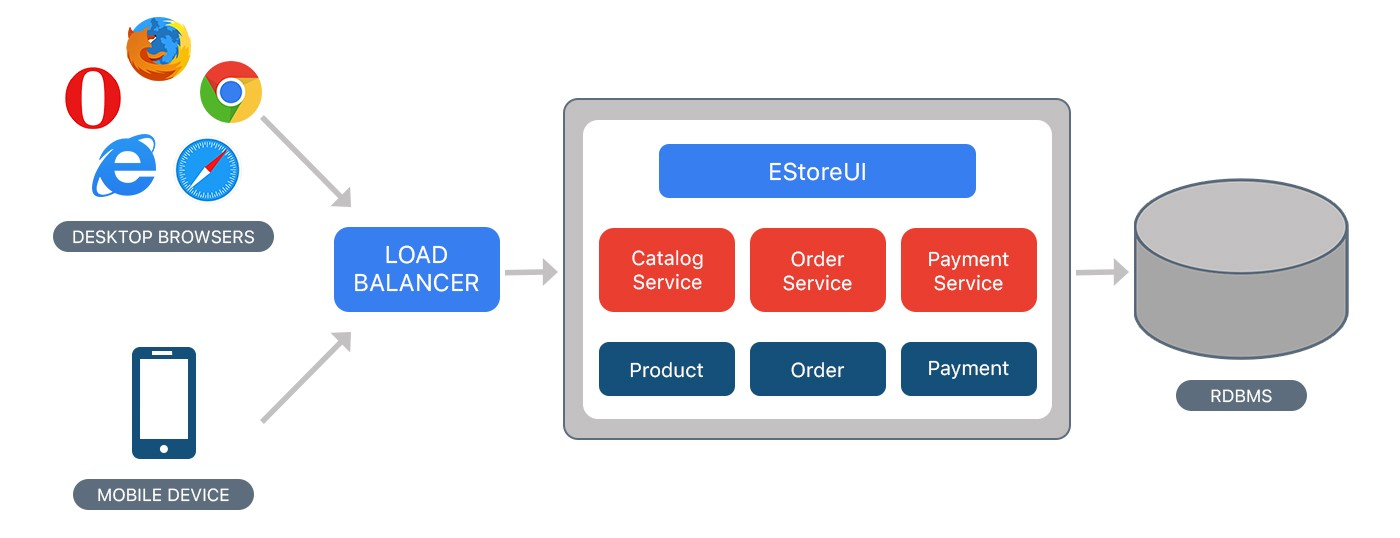
\includegraphics[width=\textwidth , keepaspectratio]{monolith.jpeg}
\centering
\caption{Esempio di \textit{monolith architecture}.}
\source{\href{https://www.medium.com/}{Medium.com}}
\label{fig:monolith}
\end{figure}

Tuttavia, questa architettura presenta alcuni -pesanti- lati negativi: innanzitutto, la velocità di avvio dell'applicazione è legata alle dimensioni della stessa, questo perché tutti i servizi vengono lanciati in un'unica volta e non \textit{on-demand}. In secondo luogo, la manutenzione del codice è resa difficile in quanto, non essendoci una netta separazione tra le varie funzionalità del prodotto, non è facile capire dove e come effettuare le modifiche richieste. Inoltre, nonostante la scalabilità orizzontale sia stata inserita tra i punti di forza di questa architettura, è presente il grosso rischio che un singolo \textit{bug}, in un qualsiasi modulo del prodotto, possa potenzialmente inibire l'intera applicazione, dato che tutte le istanze create sono identiche.
Infine, l'architettura monolitica non si presta bene all'introduzione di nuove tecnologie, dato che i cambiamenti ai linguaggi o ai \textit{framework} utilizzati andranno ad impattare su tutto il sistema, risultando quindi molto costosi e rischiosi.

%**************************************************************
\section{\textit{Stack} tecnologico}
\subsection{CakePHP}
CakePHP è un \textit{framework} in linguaggio PHP, generalmente utilizzato per la realizzazione di applicativi web.\\
Scritto in PHP, segue un approccio MVC (\textit{Model-View-Controller}) e, grazie all'\textit{ORM} integrato, facilita l'iterazione con i database relazionali. L'\textit{ORM} infatti fornisce, mediante un'interfaccia orientata agli oggetti, tutti i servizi inerenti alla persistenza dei dati, astraendo nel contempo le caratteristiche implementative dello specifico \textit{RDBMS} utilizzato. L'utilizzo di un \textit{ORM} fornisce diversi vantaggi, tra cui la diminuzione del codice sorgente da redigere, in quanto esso dispone di metodi \textit{built-in} per effettuare le operazioni più comuni (come ad esempio le \textit{CRUD}), o la gestione automatica della concorrenza nell'accesso ai dati, evitando così i conflitti tra lettura e scrittura in caso di più accessi simultanei allo stesso record.\\
Nonostante CakePHP consenta di realizzare applicazioni complete, gestendo quindi anche l'interfaccia utente, i progetti in cui sono stato inserito si appoggiano a questo \textit{framework} solamente per interfacciarsi alla base di dati tramite \textit{API}.
\subsection{MySQL e PostgreSQL}
Come detto in precedenza, in questi due progetti sono state utilizzate due basi di dati che abbracciano il paradigma SQL, rispettivamente MySQL in \DS{} e PostgreSQL in AWMS.
La principale differenza tra questi due database è la tipologia di dati memorizzabili nelle tabelle: mentre MySQL conserva tipi di dato semplici (come dati numerici, stringhe o date), PostgreSQL consente di memorizzare anche tipi di dato più complessi, come array, gli XML, oppure i JSON.
La capacità di poter memorizzare dati di tipo XML o JSON rende PostgreSQL, di fatto, una sorta di DBMS ibrido, che si frappone tra i database che utilizzano un approccio SQL puro, ed i database che invece utilizzano un paradigma NoSQL. 
\subsection{AngularJS e Angular2+}
\`E una piattaforma open source per lo sviluppo di applicazioni web sviluppato principalmente da Google. La caratteristica fondamentale di questo framework è la capacità di rendere l’applicazione eseguibile interamente lato client evitando di rispedire la pagina al server. La comunicazione con la base di dati avviene attraverso API, che viene poi gestita da CakePHP fino al ritorno del risultato richiesto.\\
\`E doveroso precisare che esistono due versioni differenti di questo \textit{framework}: \textbf{AngularJS} (anche chiamato Angular1.x) e \textbf{Angular2+}. Durante il tirocinio ho avuto modo di utilizzare entrambe le versioni, rispettivamente su \DS{} e su AWMS. 
Le differenze più evidenti si hanno nel linguaggio di programmazione, passato da Javascript ES5/ES6 a Typescript, superset tipizzato di Javascript (ES5 ed ES6 rimangono perfettamente compatibili), e nell'approccio architetturale: entrambe le versioni dichiarano una struttura MVC, ma Angular2+ utilizza una filosofia che si discosta dall'MVC classico, introducendo il concetto di \textit{Component}, ovvero il "mattone base" per la costruzione dell'applicativo.
Ogni Component applica il pattern MVC e può essere padre (o figlio) di altri Component. Questa struttura permette di trattare i singoli Component come se fossero oggetti indipendenti ed in seguito, come suggerisce il nome stesso, comporli tra loro a formare l'interfaccia.
\subsection{Redis}
Redis è un datastore in memoria molto rapido, open source e di tipo chiave-valore adatto all'utilizzo con database, caching, broker di messaggistica e code.\\
Nell'ambito dell'attività di stage, questo \textit{tool} è stato implementato solamente nel progetto AWMS, con lo scopo di salvare i risultati derivanti dalle richieste al database, così da averli immediatamente disponibili in caso di richieste multiple, rendendo il sistema più reattivo e impegnando per meno tempo la base di dati.

\begin{figure}[h]
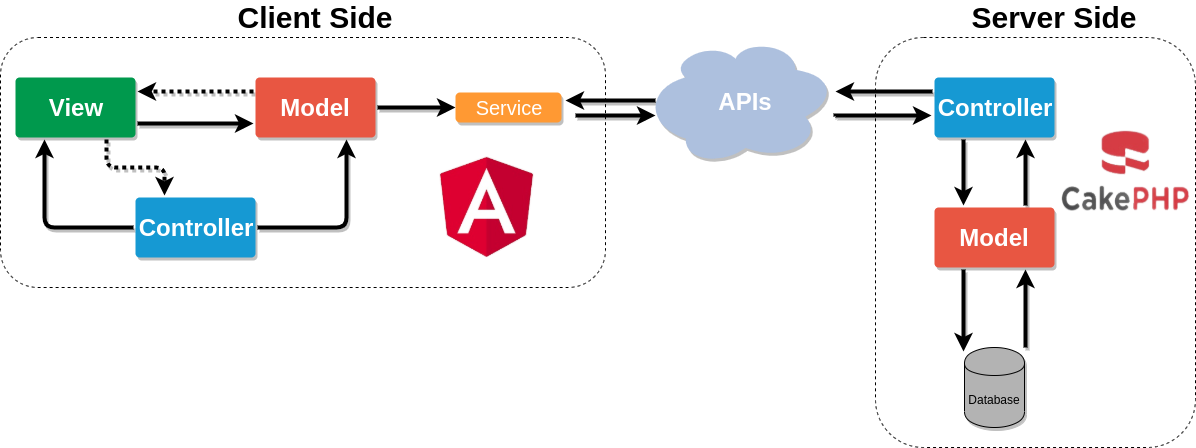
\includegraphics[width=\textwidth , keepaspectratio]{architecture.png}
\centering
\caption{Schema architetturale di come i \textit{framework} interagiscono tra loro all'interno di \DS{} ed AWMS.} 
\label{fig:architecture}
\end{figure}

%**************************************************************
\section{Pianificazione}
%pianificazione in base alle scadenze di progetto, agli sprint programmati e agli impegni accademici personali
Partecipando a due progetti già in fase di sviluppo avanzata, le attività da svolgere e le componenti da realizzare, al mio arrivo in azienda, erano chiare e ben definite. \\
Assieme al tutor aziendale, nonché responsabile dei progetti, abbiamo pianificato queste attività basandoci sulla difficoltà tecnica e sulle competenze necessarie per poterle svolgere.\\
Fissato il termine di consegna per il progetto \DS{}, coincidente con il traguardo di metà tirocinio, abbiamo quindi distribuito temporalmente le attività assegnatemi, riservando una intera settimana allo studio delle tecnologie che avrei dovuto utilizzare e alla comprensione del funzionamento del prodotto stesso.\\
Naturalmente, le attività sono state suddivise anche per progetto di appartenenza, così da rendere più ordinato (e logico) il processo di sviluppo.\\
Come descritto in §\ref{subsec:vincoli-metodologici}, il modello di sviluppo adottato è lo Scrum, che prevedeva Sprint della durata di due settimane ed un meeting di allineamento a metà di ogni Sprint, così da tenere sotto controllo l'andamento dello sviluppo ed intervenire tempestivamente in caso di eventuali difficoltà riscontrate.
Nella pianificazione, inoltre, abbiamo tenuto conto dei giorni in cui sarei stato impegnato con gli esami universitari, ma non sono state previste contromisure in caso di altre mie assenze.\\
Per quanto riguarda i rischi legati all'attività di codifica, al netto di difficoltà tecniche dovute all'inesperienza, abbiamo deciso di mitigarli tramite la stesura di test d'unità e test d'integrazione. Questa soluzione, sebbene richieda molto più tempo rispetto alla sola scrittura del codice del prodotto, consente di ridurre il rischio di introduzione di bug nel sistema.
%**************************************************************
\section{Analisi dei requisiti}
Durante questa fase, assieme al team di sviluppo, ho stilato in maniera più dettagliata i requisiti che ogni attività assegnatami doveva soddisfare.\\
Ad ogni requisito è stato quindi affidata una sigla identificativa, rendendoli così più facilmente tracciabili, e soprattutto, conferendo loro una classificazione in base all'importanza del requisito stesso.\\
La sigla identificativa di ogni requisito rispetta il formato \textbf{R[tipo][numero]}, dove la R iniziale indica che il codice si riferisce ad un requisito, "tipo" assume il valore dell'iniziale della tipologia di requisito, sia esso Opzionale, Desiderabile o Facoltativo, mentre "numero" indica il numero cardinale del requisito di tipo dato.

\subsubsection*{\DS}
In questo progetto, le mie attività erano inerenti allo sviluppo di un modulo di analisi, per cui i requisiti e le specifiche da soddisfare riguardavano prevalentemente le funzionalità e i casi d'uso relativi all'interfaccia utente.
Durante il primo \textit{meeting} con il team di sviluppo, sono stati individuati complessivamente 10 requisiti, suddivisi come segue:
\begin{itemize}
    \item \textbf{Obbligatori:} 6;
    \item \textbf{Desiderabili:} 3;
    \item \textbf{Facoltativi:} 1.
\end{itemize}
Alcuni esempi delle specifiche delineate sono riportati nella tabella a seguire.
\begin{center}
	\renewcommand{\arraystretch}{1.5}
	\rowcolors{2}{}{row}
	\begin{longtable}{ | p{0.1\linewidth} | p{0.9\linewidth} |}	 
		\hline   
	    \rowcolor{header}\textbf{Codice}&\textbf{Descrizione}\\
		\hline    	
    	RO1 & La \textit{dashboard} principale deve prevedere un sistema di filtraggio dei dati da visualizzare \\
    	RO3 & Il modulo di analisi deve permettere all'utente di selezionare la tipologia di grafico da creare \\
    	RD2 & Il modulo di analisi deve essere ben visualizzabile anche in dispositivi mobili \\
    	RF1 & Ogni utente deve poter editare solamente i progetti di cui dispone i privilegi  \\
    	\hline
		\rowcolor{white}    	
    	\caption{Tabella requisiti per il progetto \DS{}.}
	\end{longtable}
	\label{tab:requisiti-digitalsnapshots}
\end{center}
Da notare che il requisito RD2 non è stato considerato obbligatorio in quanto, per natura, l'applicazione deve consentire all'utente una panoramica sui progetti e sulle analisi. Pertanto, l'esecuzione del prodotto su dispositivi mobili, sebbene possibile, è fortemente sconsigliata.

\subsubsection*{AWMS}
Le attività da svolgere in questo progetto, invece, riguardavano la creazione di un modulo per l'esportazione di dati in forma tabellare su file di tipo PDF e/o XLSX, e si concentravano prevalentemente sul lato \textit{back-end} dell'applicativo.
Successivamente alla consegna di \DS{}, ho partecipato ad una riunione con il team di sviluppo di AWMS, nel quale abbiamo individuato 14 requisiti riguardanti le attività che mi apprestavo a svolgere, suddivisi nel seguente modo:
\begin{itemize}
    \item \textbf{Obbligatori:} 8;
    \item \textbf{Desiderabili:} 4;
    \item \textbf{Facoltativi:} 2.
\end{itemize}
Alcuni esempi delle specifiche delineate sono riportati nella tabella \ref{tab:requisiti-awms}.

\begin{center}
	\renewcommand{\arraystretch}{1.5}
	\rowcolors{2}{}{row}
	\begin{longtable}{ | p{0.1\linewidth} | p{0.9\linewidth} |}	 
		\hline   
	    \rowcolor{header}\textbf{Codice}&\textbf{Descrizione}\\
		\hline    	
    	RO1 & Il modulo di export deve permettere all'utente di selezionare il formato di file da scaricare  \\
    	RO4 & Il modulo di export deve permettere all'utente di selezionare le colonne da visualizzare nel report \\
        RO5 & Il modulo di export deve fornire all'utente un sistema di filtraggio dei dati da inserire nel report \\
    	RD1 & Il modulo di export deve fornire all'utente la possibilità di personalizzare il report in caso di stampa in formato PDF, permettendo di selezionare l'orientamento e le dimensioni dell'area di stampa\\
    	RD2 & Il modulo di export deve fornire all'utente la possibilità di inviare tramite email il file appena creato\\
    	\hline
		\rowcolor{white}    	
    	\caption{Tabella requisiti per il progetto AWMS.}
	\end{longtable}
	\label{tab:requisiti-awms}
\end{center}

% descrizione di come sono stati stilati i requisiti\\
% classificazione dei requisiti\\
% definizione dei requisiti\\
%**************************************************************
\section{Progettazione}
Successivamente all'individuazione e alla classificazione dei requisiti da soddisfare, ho potuto procedere alla fase di progettazione, nella quale ho scelto librerie e \textit{framework} di supporto, e definito una struttura che mi permettesse di soddisfare i requisiti.
\subsection{\DS}
\subsubsection{Modellazione base di dati}
Per poter raggiungere gli obiettivi prefissati, è stato necessaria un'attenta analisi della struttura e dei dati contenuti nel database. Da qui, sono emerse grosse limitazioni riguardanti la scalabilità, circoscrivendo di fatto gli ambiti di utilizzo dell'applicazione.\\
\`E stato necessario quindi ristrutturare il database, astraendo e generalizzando il più possibile le tabelle, così da rendere il prodotto più versatile nell'utilizzo. Tuttavia, a causa della prossimità della scadenza di consegna, non è stato possibile ristrutturare completamente la base di dati, ma solamente le parti alle quali mi sono approcciato.   
\subsubsection{Progettazione API}
Una volta definita la struttura del database, ho provveduto predisporre gli \textit{endpoint} per le richieste HTTP che il client dovrà effettuare per poter accedere ai dati.\\
Prima di progettare la realizzazione di un nuovo \textit{endpoint}, mi sono assicurato che non ce ne fossero altri che avevano lo stesso scopo, così da evitare di duplicare il codice ed aumentare la complessità del prodotto. Questa attività è stata molto onerosa in termini di tempo a causa della scarseggiante documentazione del codice, che mi ha obbligato quindi ad una revisione manuale dell'intero progetto.
\begin{figure}[h]
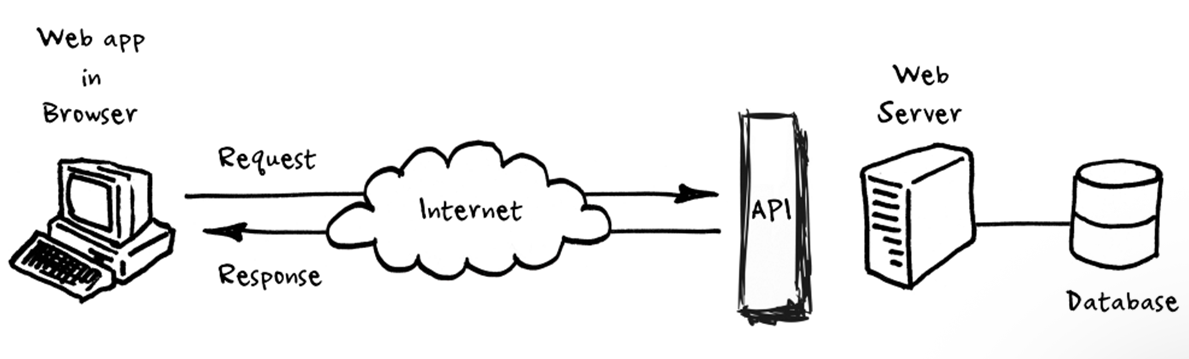
\includegraphics[width=\textwidth , keepaspectratio]{api-simple.png}
\centering
\caption{Semplificazione del funzionamento di una API REST.} 
\label{fig:api-simple}
\end{figure}
%- architettura REST, quindi importanza delle API\\
%- progettazione e descrizione API più significative\\
\subsubsection{Progettazione interfaccia utente}
Per quanto riguarda l'impostazione e lo stile dell'interfaccia utente, non ho dovuto progettare più di tanto, in quanto ero vincolato a seguire i \textit{mockup} realizzati (e già approvati dagli \textit{stakeholder}) dal UI/UX designer.\\
Per la realizzazione dei grafici ho sfruttato la libreria open source Chart.Js\footnote{\textit{Chart.Js.} URL: \href{https://www.chartjs.org/}{https://www.chartjs.org/}}, che permette la facile implementazione di diverse tipologie di grafico, mantenendo la struttura dei dati in ingresso pressoché invariata tra un tipo di grafico e l'altro. 
Questa caratteristica mi ha permesso di standardizzare la creazione del grafico applincando un \textit{factory pattern}, quindi estendendo la classe \textit{Chart}, fornita dalla libreria, ed implementando dei metodi di servizio per la selezione della tipologia di grafico, per l'aggiunta di ulteriori \textit{dataset} (ove possibile) o per la modifica delle opzioni di rendering.
\begin{figure}[h]
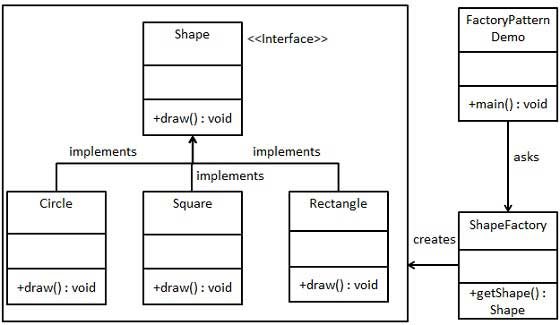
\includegraphics[width=\textwidth , keepaspectratio]{factory_pattern_uml_diagram.jpg}
\centering
\caption{Esempio di \textit{factory pattern}.}
\source{\href{https://www.tutorialspoint.com/design_pattern/factory_pattern.htm}{Tutorialspoint.com}}
\label{fig:factory-pattern}
\end{figure}

%- da mockup a GUI\\
%- limitazioni applicative (per natura della webapp => poco responsive e poca accessibilità)\\

\subsection{AWMS}
\subsubsection{Modellazione base di dati}
Dal punto di vista del DBMS, AWMS è molto più strutturato rispetto a \DS{}. Parte del merito è riconducibile all'utilizzo di PostgreSQL che, grazie alla sua capacità di immagazzinare dati in formato JSON, consente agli sviluppatori di creare delle colonne temporanee nelle quali inserire e testare i nuovi dati da implementare. Una volta verificata l'utilità di tali dati, verrà creata una colonna apposita per tipologia di dato in aggiunta e verranno quindi rimossi dalla colonna temporanea.\\
Le modifiche che ho apportato a questo DBMS sono state molto limitate e si è trattato esclusivamente di aggiunte di nuove colonne, come ad esempio l'orario di inizio e di fine della pausa pranzo dello staff, o gli indirizzi di posta elettronica ai quali inviare la pianificazione giornaliera.  
%- importanza di una buona progettazione del db\\
%- modifiche apportate alle basi di dati\\
\subsubsection{Progettazione API e generazione dei report}
Fortunatamente, la progettazione delle API per la stampa è stata semplificata dal fatto che ho potuto riutilizzare le \textit{query} create per la visualizzazione a schermo della pianificazione giornaliera. \\
Per quanto concerne la creazione del report di stampa, ho scelto di appoggiarmi alla libreria PHPSpreadsheet\footnote{\textit{PHPSpreadsheet.} URL: \href{https://phpspreadsheet.readthedocs.io/en/latest/}{https://phpspreadsheet.readthedocs.io/}} per la generazione del file in formato XLSX, e a TCPDF\footnote{\textit{TCPDF.} URL: \href{https://tcpdf.org/}{https://tcpdf.org/}} per la generazione del file in formato PDF.\\
Dopo uno studio approfondito e qualche prova in ambiente \textit{sandbox} di entrambe le librerie, ho individuato gli \textit{step} comuni per arrivare alla generazione dei file, riuscendo così ad incapsulare i due algoritmi dentro un pattern di tipo \textit{template method}.\\
\begin{figure}[h]
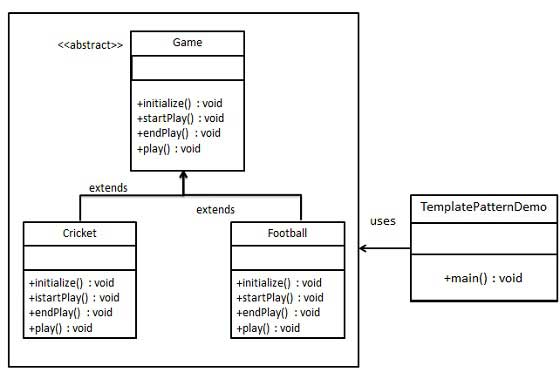
\includegraphics[width=\textwidth , keepaspectratio]{template_pattern_uml_diagram.jpg}
\centering
\caption{Esempio di \textit{template method pattern}.}
\source{\href{https://www.tutorialspoint.com/design_pattern/template_pattern.htm}{Tutorialspoint.com}}
\label{fig:template-pattern}
\end{figure}

Per quanto concerne il filtraggio dei dati da stampare, ho strutturato un \textit{filter pattern}, così da rendere più dinamica la creazione ed applicazione di filtri. \\
\begin{figure}[h]
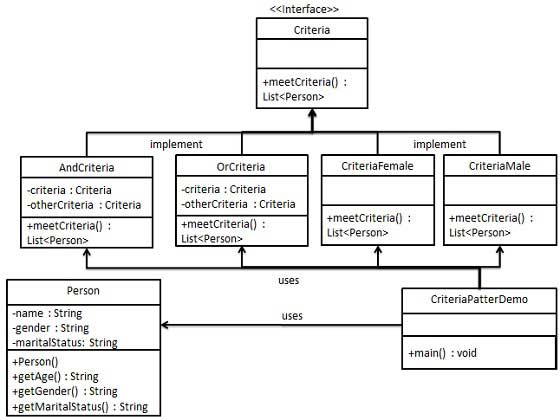
\includegraphics[width=0.9\textwidth , keepaspectratio]{filter_pattern_uml_diagram.jpg}
\centering
\caption{Esempio di \textit{filter pattern}.}
\source{\href{https://www.tutorialspoint.com/design_pattern/filter_pattern.htm}{Tutorialspoint.com}}
\label{fig:filter-pattern}
\end{figure}
%- architettura REST, quindi importanza delle API\\
%- progettazione e descrizione API più significative\\

\subsubsection{Progettazione interfaccia utente}
Anche in questo caso, l'interfaccia utente non ha avuto bisogno di molta progettazione, in quanto dovevo seguire quanto esplicitato nel \textit{mockup} creato dai designer.
%**************************************************************
\section{Codifica}
In seguito alla progettazione dell'architettura e dei componenti dei progetti in questione, sono passato alla fase codifica.\\
Lo sviluppo, nonostante l'inesperienza, è avanzato senza troppe difficoltà tecniche, questo anche dovuto al fatto che le attività assegnatemi erano relativamente semplici o comunque di contorno. Inoltre, in caso di dubbi, potevo sempre contare sull'aiuto dei colleghi, che si sono rivelati molto disponibili nell'aiutarmi.\\
Le maggiori difficoltà, tuttavia, le ho incontrate durante le attività di modifica al database e nel \textit{refactoring} di alcuni metodi già esistenti, come ad esempio le \textit{query} per il recupero dei dati richiesti. Ciò è stato causato dalla quasi totale assenza, in entrambi i progetti, di documentazione riguardante la struttura della base di dati e delle funzionalità del codice scritto fino a quel momento. 

\begin{figure}[h]

\includegraphics[width=\textwidth , keepaspectratio]{bad-coding-issues.jpeg}
\centering
\caption{Conseguenze di una cattiva codifica e dell'assenza di documentazione.} 
\source{\href{https://medium.com/better-programming/good-code-vs-bad-code-35624b4e91bc}{Medium.com}}
\label{fig:bad-coding-issues}
\end{figure}
%\subsection{Implementazione moduli di stampa}
%- stampa su file .xlsx e/o .pdf\\
%- front-end => dialog con scelta di opzioni di stampa\\
%- back-end => design pattern applicati e principi SOLID\\
%\subsection{Implementazione cruscotti delle analisi}
%\begin{figure}[h]
%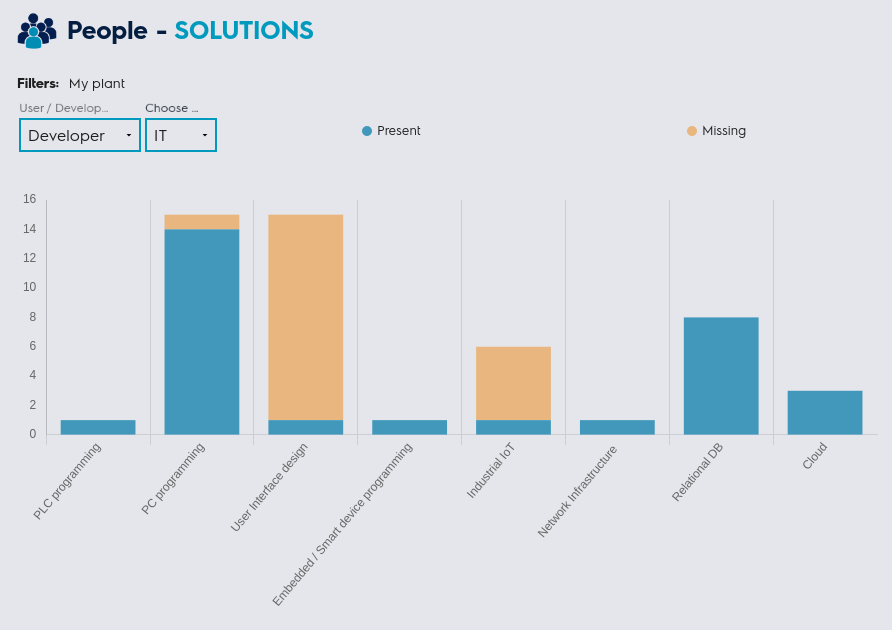
\includegraphics[width=\textwidth , keepaspectratio]{grafico-developers.png}
%\centering
%\caption{Esempio di grafico realizzabile nella piattaforma \DS{}.} 
%\label{fig:grafico-developers}
%\end{figure}
%- importanza dei cruscotti di analisi
%- implementazione libreria chart.js
%**************************************************************
\section{Verifica}
\subsection{Analisi statica}
In entrambi i progetti alla quale ho partecipato, abbiamo effettuato l'analisi statica del codice utilizzando delle apposite librerie che permettono di verificare se il codice rispetta le regole standard del linguaggio utilizzato, oltre che consentire di configurare preferenze e personalizzazioni stilistiche.
Nello specifico, abbiamo utilizzato ESLint per l'analisi del codice basato su Javascript (quindi anche per Typescript), mentre per il codice PHP ci siamo affidati alle librerie PHP Parallel Lint, CodeSniffer e PHPStan, utili rispettivamente per il controllo della sintassi, dello stile e degli errori logici.\\
Purtroppo, nessuno dei due progetti era provvisto di \textit{continous integration}, quindi questi controlli venivano effettuati solamente nell'ambiente di sviluppo locale, non assicurando la conformità del codice redatto dai membri dei team, alle norme configurate in questi \textit{tool}.
\subsection{Analisi dinamica}
L'attività di analisi dinamica è stata effettuata tramite l'esecuzione automatica dei test sviluppati prima della stesura del codice del prodotto, seguendo l'approccio TDD (Figura \ref{fig:tdd}).\\
L'ambiente di testing consiste in una \textit{pipeline} automatica configurata tramite il \textit{framework} Jenkins. Data l'assenza della \textit{continous integration} in entrambi i progetti, la \textit{pipeline} è stata configurata solamente in ambiente locale, così da poter testare e sperimentare senza correre il rischio di entrare in conflitto con l'ambiente di produzione.\\
La struttura dei test da effettuare è stata generata automaticamente dai \textit{plug-in} di PHPUnit (per il codice PHP) e Jasmine (per il codice Javascript/Typescript), installati nell'IDE PHPStorm. Questa funzionalità mi ha permesso di risparmiare molto tempo, in quanto ho dovuto solamente codificare il corpo del test da eseguire.\\
Di seguito riporto i risultati di alcuni test effettuati nel progetto AWMS, come esempio:

\begin{center}
	\renewcommand{\arraystretch}{1.5}
	\rowcolors{2}{}{row}
	\begin{longtable}{ | p{0.1\linewidth} | p{0.8\linewidth} | p{0.1\linewidth}|}	 
		\hline   
	    \rowcolor{header} \textbf{Codice} & \textbf{Descrizione} & \textbf{Esito}\\
		\hline    	
    	TU1 & Il componente stampa il logo di \AD{} nel caso in cui non sia stato caricato un logo aziendale & Superato  \\
    	TU2 & Il componente, se non trova il dato richiesto, gestisce l'eccezione stampando '-' nella cella corrente & Superato \\
        TU3 & Il componente stampa correttamente i campi selezionati nelle opzioni di stampa & Superato \\
    	TU4 & Il componente evidenzia correttamente lo staff non pianificato & Superato\\
    	TU5 & Il componente effettua correttamente l'unione dei record in caso di pianificazioni consecutive e di selezione dell'opzione & Superato\\
    	\hline
		\rowcolor{white}    	
    	\caption{Tabella dei test di unità per il progetto AWMS.}
	\end{longtable}
	\label{tab:unit-test-awms}
\end{center}
Nonostante il superamento di tutti i test eseguiti in locale, questa tipologia di analisi dinamica non deve essere considerata affidabile, in quanto sono stati effettuati dei test di sistema in maniera manuale e molto poco approfondita. Questa cattiva pratica purtroppo, non solo potenzialmente vanifica quanto fatto in precedenza, ma espone l'applicazione a grossi rischi di affidabilità, come descritto in §\ref{subsec:architettura-monolitica}. 
%- creazione dei test prima della codifica (TDD)\\
%- classificazione dei test\\
%- esecuzione automatica dei test d'unità e di integrazione. Test di sistema effettuati manualmente \\
%- framework utilizzati: phpUnit per back-end, karma/jasmine per front-end\\
%**************************************************************
\section{Validazione}
\subsection{Bilancio dei requisiti soddisfatti}
Terminata la fase di sviluppo, siamo passati alla fase di verifica della copertura dei requisiti, accertandoci quindi che il prodotto finale rispondesse alle esigenze richieste.\\
Per entrambi i progetti, il bilancio risulta essere positivo: sono stati da me soddisfatti tutti i requisiti obbligatori ed alcuni desiderabili.\\
Per quanto concerne il progetto \DS{}, non sono stati soddisfatti i requisiti:
\begin{itemize}
    \item \textbf{RD2:} nonostante l'interfaccia sia \textit{responsive}, il modulo di analisi non è ben visualizzabile da dispositivi di piccole dimensioni, a causa della grande varietà di dati analizzati, che rende un po' confusionaria la schermata.  
    \item \textbf{RF1:} l'implementazione di una gerarchia di utenti con livelli di privilegi diversi, avrebbe richiesto troppo tempo e una ri-progettazione di quasi tutto il database. Per questo motivo abbiamo deciso di trascurare questo requisito.
\end{itemize}
Nell'ambito del progetto AWMS invece, la copertura dei requisiti soddisfatti risulta essere del 100\%{}, segno di un'ottima fase di pianificazione e progettazione, che hanno permesso alla fase di codifica di essere puntuale con le scadenze fissate, nonostante il poco tempo a disposizione.
\subsection{Visione d'insieme}
Nel complesso, i team di sviluppo con i quali ho collaborato, si sono detti soddisfatti del lavoro svolto, tanto che mi è stato proposto di continuare a lavorare in \AD{} dopo la laurea.\\
\begin{figure}[h]
\centering
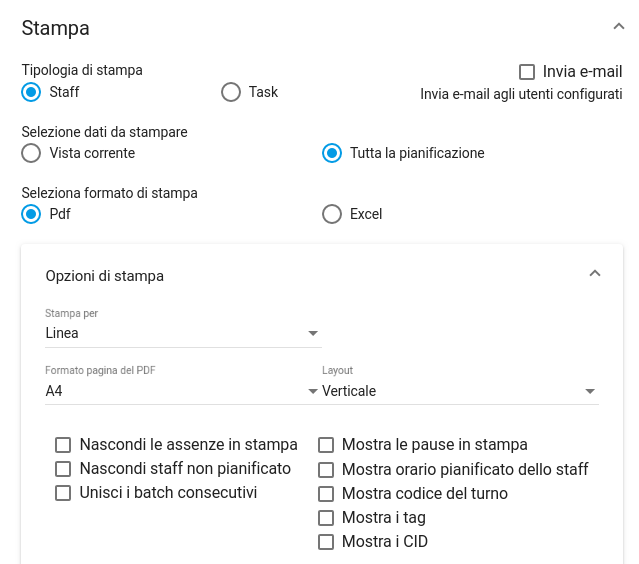
\includegraphics[width=0.8\textwidth]{interfaccia-stampa-awms.png} 
\caption{Interfaccia per la stampa della pianificazione giornaliera di AWMS.}
\end{figure}

Per quanto riguarda la consegna di \DS{}, il reparto tecnico di Electrolux ha fornito un feedback positivo sul modulo di analisi che ho implementato, abbozzando la possibilità che la stessa struttura possa essere implementata in altri progetti interni. 
\begin{figure}[h]
\centering
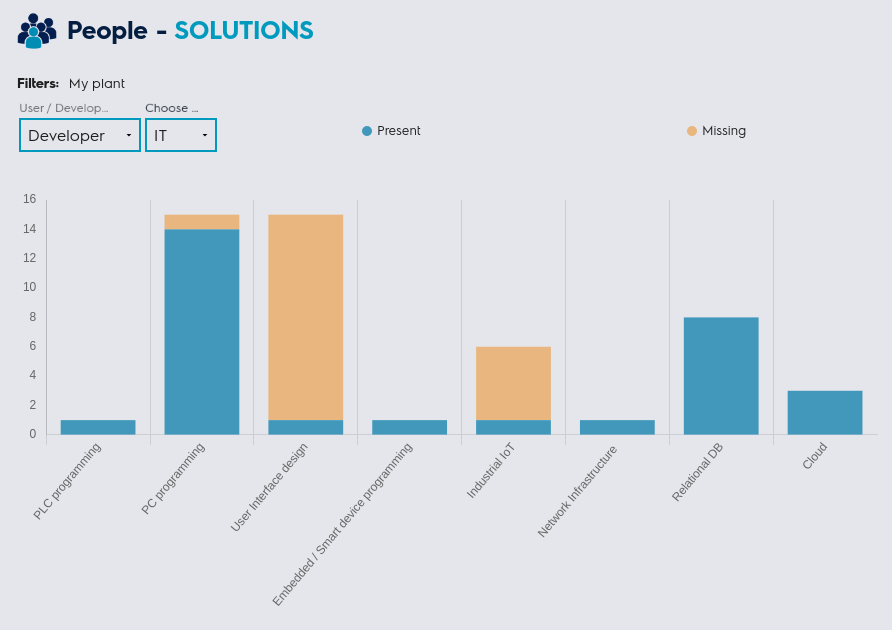
\includegraphics[width=0.8\textwidth]{grafico-developers.png} 
\caption{Esempio di grafico realizzabile tramite il modulo di analisi implementato in \DS{}.}
\end{figure}

%bilancio dei requisiti soddisfatti\\
%**************************************************************